\documentclass{report-UTC}

\usepackage[hidelinks]{hyperref}
\setlength{\parindent}{0pt}

\UV{AI23} 
\title{Rapport projet A23}
\author{{\sc Petrel} Lucas $|$ {\sc Zizouni} Maher \\ {\sc Mougoue} Ruben $|$ {\sc Anière} Quentin}


\begin{document}

\thispagestyle{empty}
\setcounter{page}{0}

\begin{figure}[H]
\centering

\includegraphics[width=7cm]{./logo_utc.pdf}
\end{figure}

\vspace{3cm}

\begin{center}

{\color{jauneUTC}\rule{\linewidth}{0.8mm}}
\vspace*{0mm}

\Huge{\textbf{\theUV \\ \thetitle}}
{\color{jauneUTC}\rule{\linewidth}{0.8mm}}

\vspace{0.5cm}
\Large{
    \sc{Petrel} Lucas \\
    \sc{Zizouni} Maher \\
    \sc{Mougoue} Ruben \\
    \sc{Anière} Quentin
} \\

\vspace{7cm}

\Large{25 décembre 2023}
\end{center}
 
\vspace{3cm}

\pagebreak

\tableofcontents{}

\pagebreak

\section{Présentation du projet}
\subsection{Contexte}

Ce projet a été réalisé dans le cadre de l'UV AI23 / NF16 à l'UTC. Il 
consiste en la conception et la réalisation d'une base de données pour
une bibliothèque. Les technologies utilisées sont le langage SQL, le SGBD
PostgreSQL et le langage Python pour l'application.

\subsection{Organisation du projet}

Le projet par 4 personnes et a été divisé en 5 jalons. Chaque jalon est déposé 
sur le dépôt Gitlab de l'UTC. 

\subsection{Note de clarification et première version du MCD}

Le premier jalon a consisté à clarifier le sujet et à réaliser une première
version du MCD. Cette version a été réalisée en groupe et a été déposée sur
le dépôt Gitlab. Nous avons utilisé \textit{plantuml} pour le MCD, il a l'avantage
d'être au format texte et donc facilement modifiable par plusieurs personnes
avec un outil de versionning comme Git.

La première version du MCD est disponible en annexe.

\subsection{Correction du MCD et MLD}

Suite aux commentaires reçus sur le premier MCD, nous avons réalisé une seconde
version du MCD. Les corrections concernaient principalement sur un problème de
de relation (composition au lieu d'agrégation) ainsi que le rajout de la 
date de retour d'un prêt.

Nous avons ensuite transformé le MCD en MLD. Nous avons rencontré quelques
difficultés au niveau du choix du type d'héritage pour les tables, nous avons 
finalement choisi l'héritage par classe mère.

La deuxième version du MCD est disponible en annexe.

\subsection{Code SQL}
\subsubsection{Création des tables}

Nous avons converti le MLD en code SQL pour créer les tables. Nous avons pas 
rencontré de difficultés particulières pour cette partie, appart le fait que 
nous avons du créer les tables dans un ordre précis pour éviter les problèmes
de dépendances.

\subsubsection{Création des vues}

Nous avons créé les vues en nous basant sur les requêtes SQL demandées dans le
sujet. Nous avons pas rencontré de difficultés particulières pour cette partie.

Les vues permettent de simplifier l'utilisation de la base de données pour
l'application Python et d'améliorer les performances.

\subsubsection{Insertion des données}

Nous avons inséré les données dans les tables. Nous avons pas rencontré de
difficultés particulières pour cette partie si ce n'est que nous avons du
insérer les données dans un ordre précis pour éviter les problèmes de
dépendances (comme lors de la création des tables).

\subsection{Application Python}

Nous avons réalisé une application Python pour utiliser la base de données.
Nous avons utilisé la librarie \textit{psycopg2} pour communiquer avec la base
de données. Nous avons choisi le format web pour notre application, avec la 
librairie \textit{flask}. Cette application est documentée dans la prochaine 
section.    

\section{Documentation de l'application}
\subsection{Archictecture}

Nous avons choisi de faire une application web pour utiliser la base de données
car c'est le format le plus simple à utiliser et le plus pratique pour ce type
d'application. Nous avons utilisé la librairie \textit{flask} pour le serveur
web (backend) et \textit{psycopg2} pour communiquer avec la base de données. \\

Pour la partie interface, c'est tout simplement du HTML/CSS/JS. Nous avons
utilisé \textit{tailwindcss} pour du style CSS déjà prêt. Les deux communiquent
avec une API REST. Nous avons utilisé l'outil \textit{swagger} pour documenter
l'API.

\begin{figure}[H]
\centering
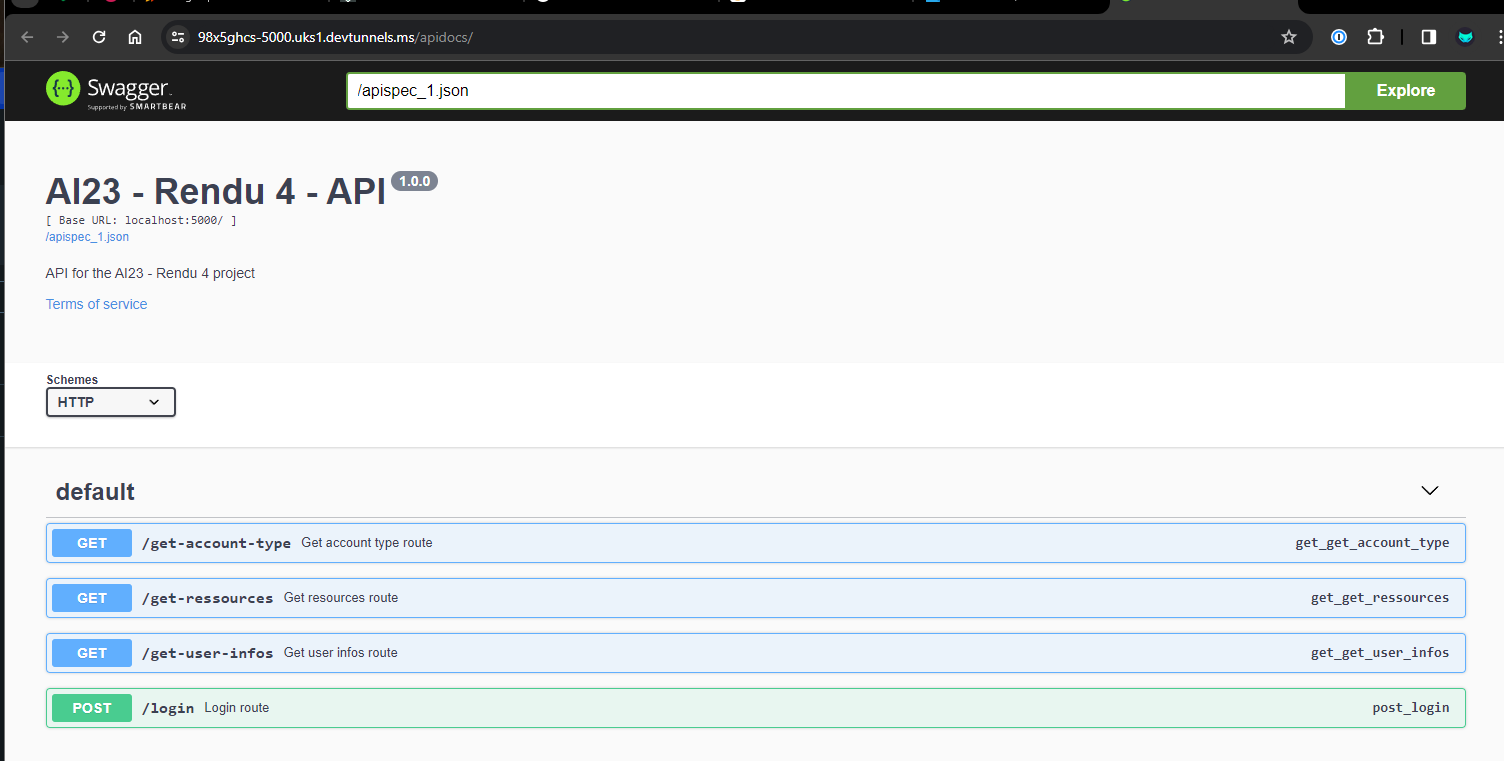
\includegraphics[width=15cm]{./images/swagger.png}
\caption{Documentation de l'API}
\end{figure}

\subsection{Partie backend}

Le backend est composé de 2 fichiers : 

\begin{itemize}
    \item \textit{app.py} : le fichier principal qui contient le serveur web
    \item \textit{database.py} : le fichier qui contient les fonctions pour communiquer
    avec la base de données
\end{itemize}

\subsubsection{app.py}

Ce fichier contient le serveur web. Il associe une route (URL) à une fonction.
Cette fonction va communiquer avec la base de données et renvoyer le résultat
au format JSON. \\

Nous avons utilisé la librairie \textit{flask} pour le serveur web. Nous avons
utilisé la librairie \textit{psycopg2} pour communiquer avec la base de données.
Nous avons utilisé la librairie \textit{flask-cors} pour permettre à l'application
web d'accéder à l'API. \\

Nous avons utilisé la librairie \textit{flasgger} pour documenter l'API. Cette
librairie permet de générer une documentation au format \textit{swagger} à partir
des commentaires dans le code. \\

Nous avons utilisé la librairie \textit{python-dotenv} pour charger les variables
d'environnement depuis un fichier \textit{.env}. 

\subsubsection{database.py}

Ce fichier contient les fonctions pour communiquer avec la base de données. Nous
avons utilisé la librairie \textit{psycopg2} pour communiquer avec la base de 
données. \\

Nous avons créé une fonction pour chaque requête SQL. L'intêret d'avoir 
un ficher dédié est de pouvoir changer d'interface facilement (par exemple
passer d'une interface web à une interface en ligne de commande). \\

\subsection{Partie frontend}

Le frontend est composé de 2 fichiers HTML :

\begin{itemize}

    \item \textit{login.html} : la page qui permet de se connecter à l'application
    \item \textit{dashboard.html} : la page d'accueil de l'application

\end{itemize}

Nous avons également trois fichiers HTML, des vues qui sont intégrés dans la 
page \textit{dashboard.html} avec un \textit{iframe} :

\begin{itemize}

    \item \textit{catalog.html} : la page qui affiche toute les ressources 
    de la bibliothèque et qui permet d'emprunter.
    \item \textit{adherents.html} : la page qui permet de gérer les membres
    \item \textit{creer\_adh.html} : la page qui permet de créer un nouveau
    membre.
\end{itemize}

Nous avons utilisé la librairie \textit{tailwindcss} pour le style CSS. Cela
permet de gagner du temps avec des classes CSS déjà prêtes. La communication
avec le backend se fait avec l'API REST. Nous avons utilisé la fonction
standard \textit{fetch} pour communiquer avec l'API. \\

L'authefication se fait avec un token JWT (JSON Web Token). Ce token est généré
lors de la connexion et est stocké dans le local storage du navigateur. Il est
ensuite envoyé dans le header de chaque requête. Cela permet de vérifier que    
l'utilisateur est bien connecté a chaque requête. \\

Des captures d'écran de l'application sont disponibles en annexe.

\section{Annexes}
\subsection{MCD (Version 1)}

\begin{figure}[H]
\centering
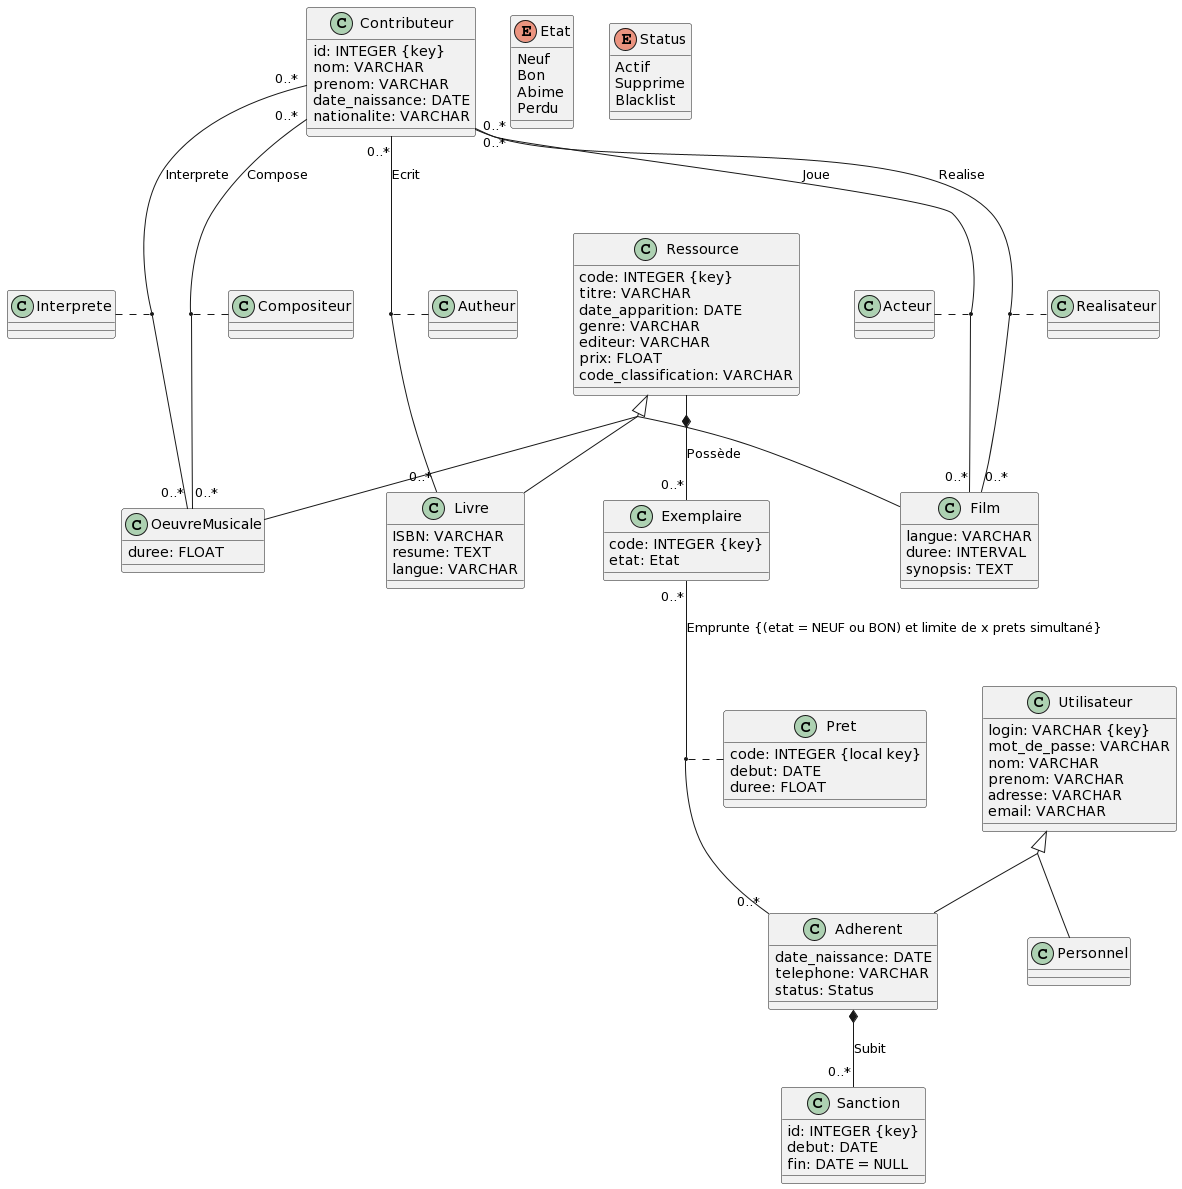
\includegraphics[width=15cm]{../Rendu1/mcd.png}
\caption{Première version du MCD}
\end{figure}

\subsection{MCD (Version 2)}

\begin{figure}[H]
\centering
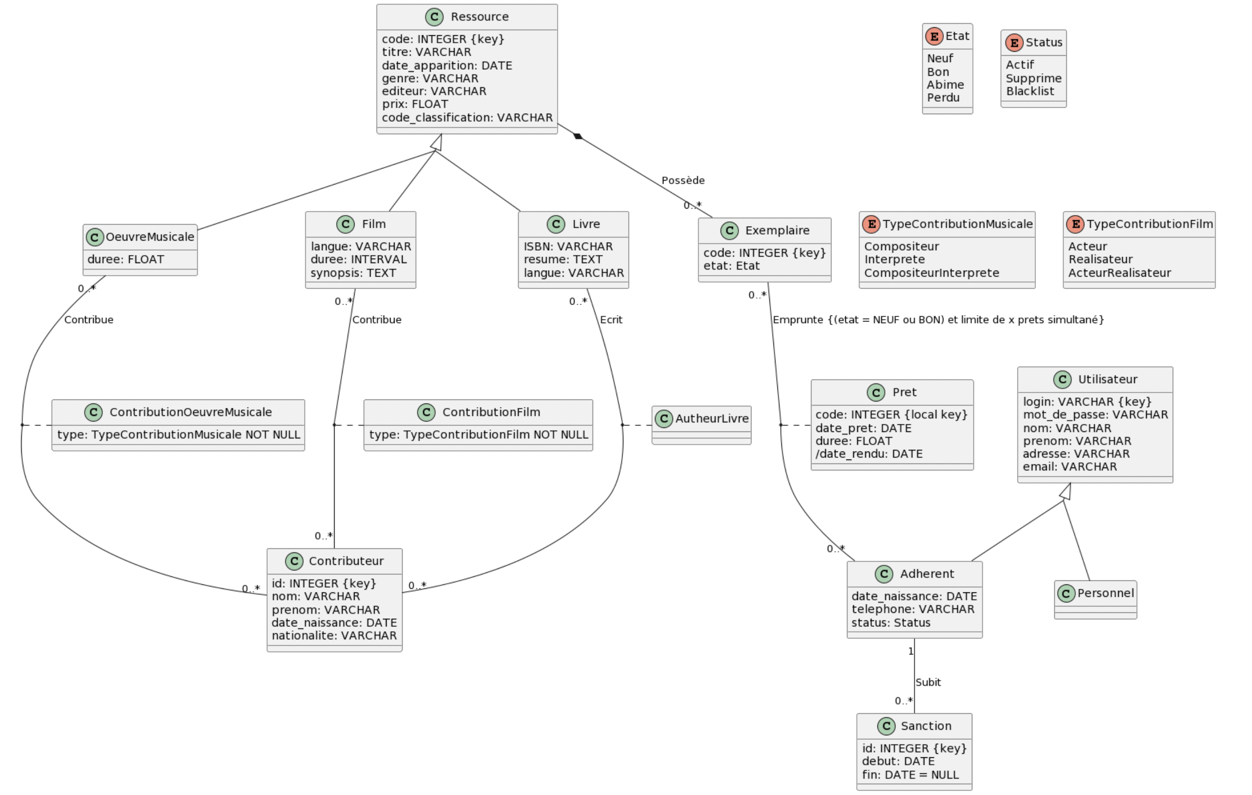
\includegraphics[width=15cm]{../Rendu2/mcdV2.png}
\caption{Deuxième version du MCD}
\end{figure}

\subsection{Captures d'écran de l'application}

\begin{figure}[H]
\centering
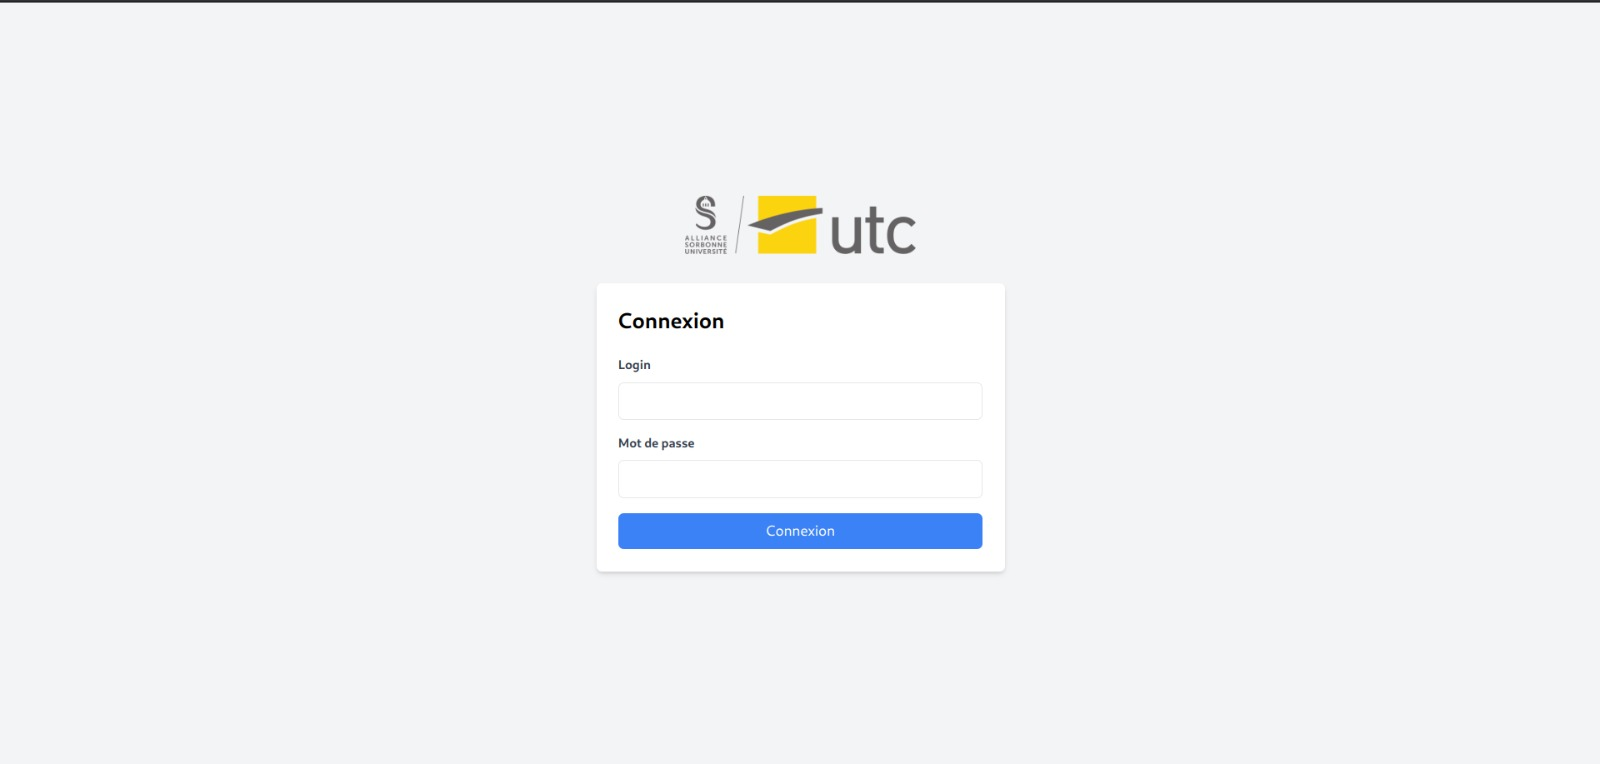
\includegraphics[width=15cm]{./images/login.jpeg}
\caption{Page de connexion}
\end{figure}

\begin{figure}[H]
\centering
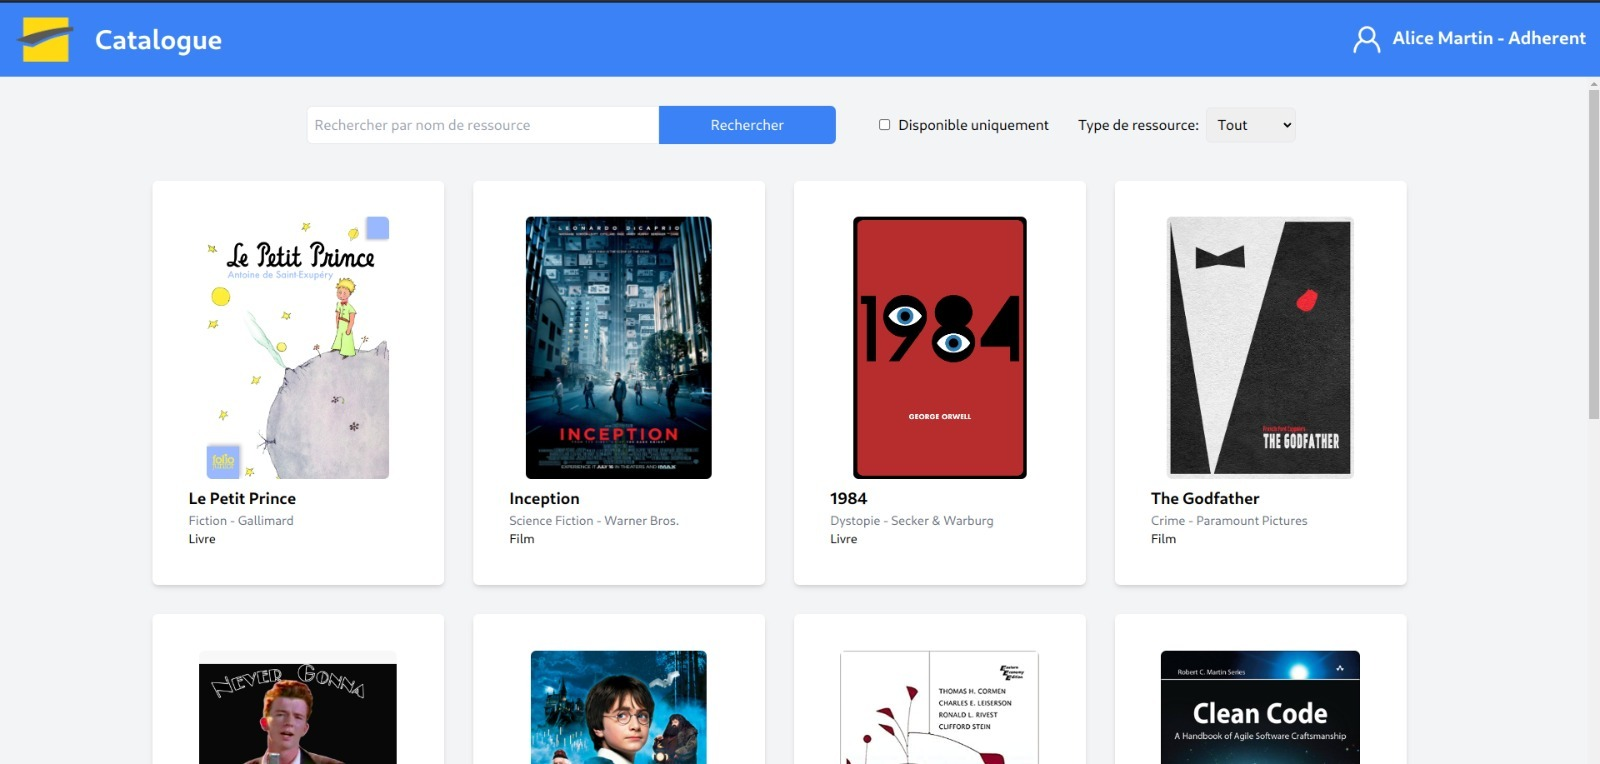
\includegraphics[width=15cm]{./images/dashboard.jpeg}
\caption{Page d'accueil}
\end{figure}

\begin{figure}[H]
\centering
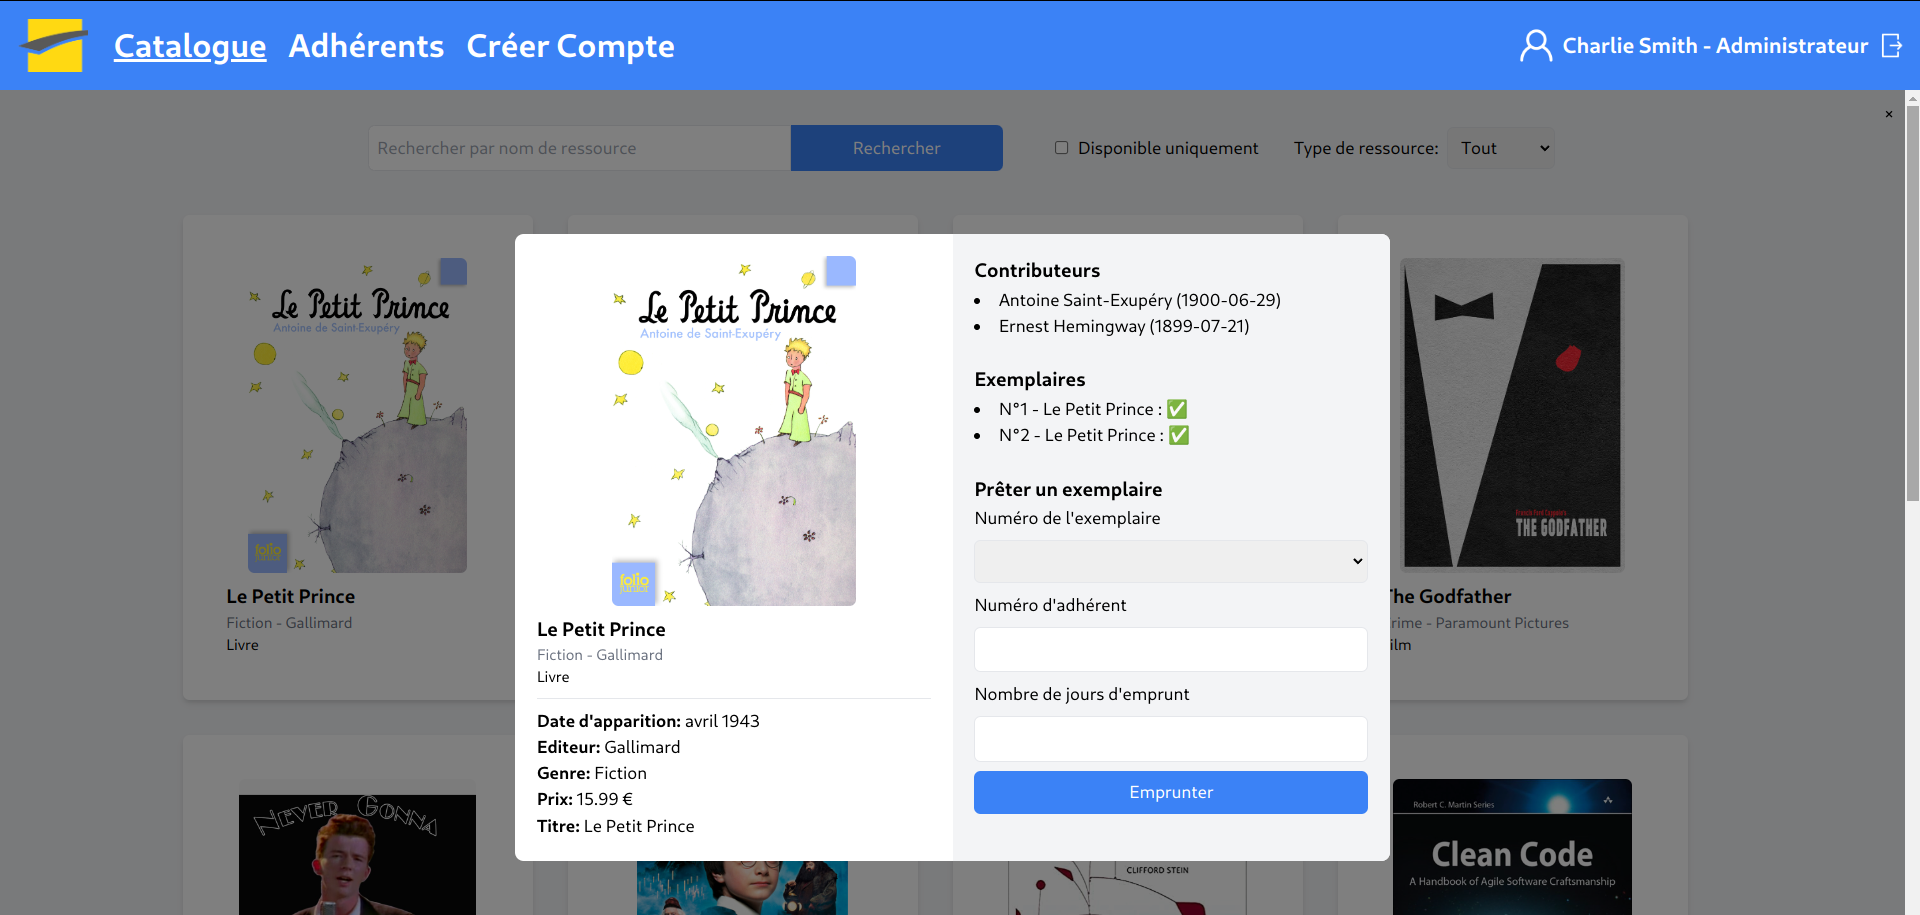
\includegraphics[width=15cm]{./images/emprunt.png}
\caption{Page d'emprunt}
\end{figure}

\end{document}